\subsection{Data From SMC}
Above in \myref{sec:queries} we discussed different queries relevant for collecting data from the schedule, here we will illustrate what this data may look like, and discuss the usefulness thereof.
We will in particular focus on the queries with keyword \textit{simulate}, as they are included for the purpose of extracting data.
When the tool is executed by the user, $100$ simulations of these queries will be run, but for the purpose of this section fewer will be run in order to better visualise the data. 

\begin{figure}[h]
	\centering
	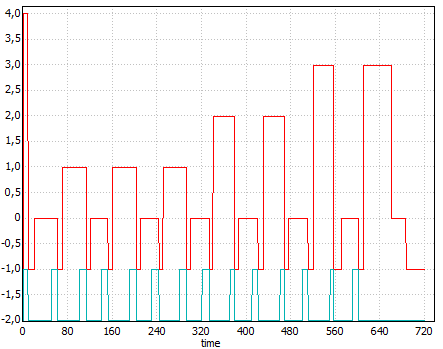
\includegraphics[scale=0.8]{graphics/active_running.png}
	\caption{Result of running query \ref{eq:smc4} in the UPPAAL GUI}
	\label{fig:active_running}
\end{figure}
First consider query \ref{eq:smc4}, this will result in a graph showing what payloads was supposed to run and when they would start and end, and whether or not they actually were executed.
We have run this query through the UPPAAL GUI which generates a graph based on the result. 
The graph can be seen in \cref{fig:active_running}.
It should be noted that such graphs are not made available to the user via our tool, but all of the values needed to make such a graph is saved and made available to the user.

We can see in \cref{fig:active_running} that all payloads are executed except for the last two.
This can be seen by looking at the parts where the red curve is different from $-1$, if the blue curve at any time in these periods differs from $-2$ it means that the payload was executed.\\
The reason for the last two not being executed, is that executing them would result in depletion of the available charge, as can be seen in \cref{fig:sim5a} on the left. 

\begin{figure}[h]%
	\centering
	\subfloat
	{{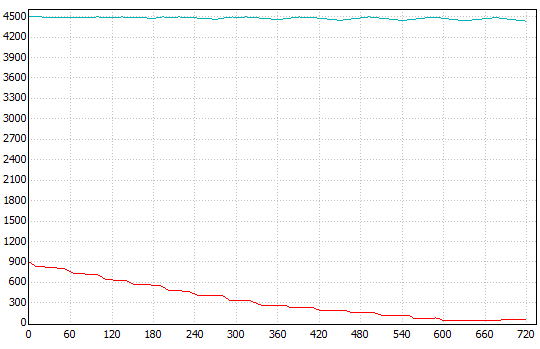
\includegraphics[width=7cm,,clip] {graphics/simAB1.png} }}%
	\qquad
	\subfloat
	{{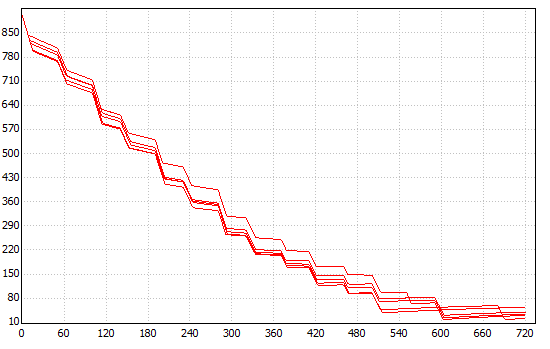
\includegraphics[width=7cm,clip] {graphics/sim5A.png} }}%
	\caption{1 simulation of \uppVar{a} and \uppVar{b}(left) 5 simulations of \uppVar{a}(right)}%
	\label{fig:sim5a}%
\end{figure}
On the left in \cref{fig:sim5a} we see the battery charges available(red), and bound(blue), over one simulation.
For this example the starting capacity is $900$ for available and $4500$ for bound.
It can be seen that the bound charge is relatively stable, meaning its capacity does not vary much, whereas the available charge gets close to depletion, resulting in the last two payloads in \cref{fig:active_running} being skipped.\\
In \cref{fig:sim5a} on the right the available charge, \uppVar{a}, have been simulated five times.
This shows some interesting results, for some of the simulations the same skips occur as in \cref{fig:active_running} i.e. the last two, whereas some simulations result in the very last payload being executed but the two prior to it being skipped.
This is a result of the feature in the \gls{smc} model that allows execution times of payloads to vary, and thus consume more or less power.
